\documentclass[11pt]{article}
\usepackage[utf8]{inputenc}
\usepackage{polski}
\usepackage{geometry}
\newgeometry{tmargin=1.5cm, bmargin=1.5cm, lmargin=1.5cm, rmargin=1.5cm}
\usepackage{graphicx}
\graphicspath{ {./img/} }
\usepackage{wrapfig}
\usepackage{listings}
\usepackage{float}

\title{CPS - Laboratoria}

\begin{document}

\maketitle

\section{Efekt Gibbsa}
Efekt "przerzutów"/ oscylacji w miejscach nieciągłości funkcji odtworzonej za pomocą szeregu Fouriera. Można go zmniejszyć zwiększając liczbę współczynników szeregu jednak nie można go wyeliminować - jego minimalna wartość to około 9\%. 

\begin{figure}[h]
    \centering
    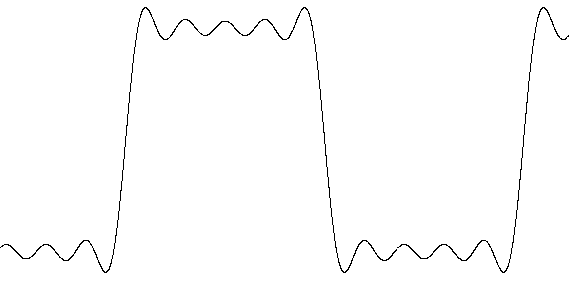
\includegraphics[width=6cm]{gibbs.png}
\end{figure}

\section{Próbkowanie i odtwarzanie sygnału analogowego}
Próbkowanie sygnału powoduje powstanie kopii jego oryginalnego widma w dziedzinie częstotliwości. Kolejne kopie są przesunięte w dziedzinie częstotliwości o kolejne wielokrotności częstotliwości próbkowania.
\begin{figure}[h]
    \centering
    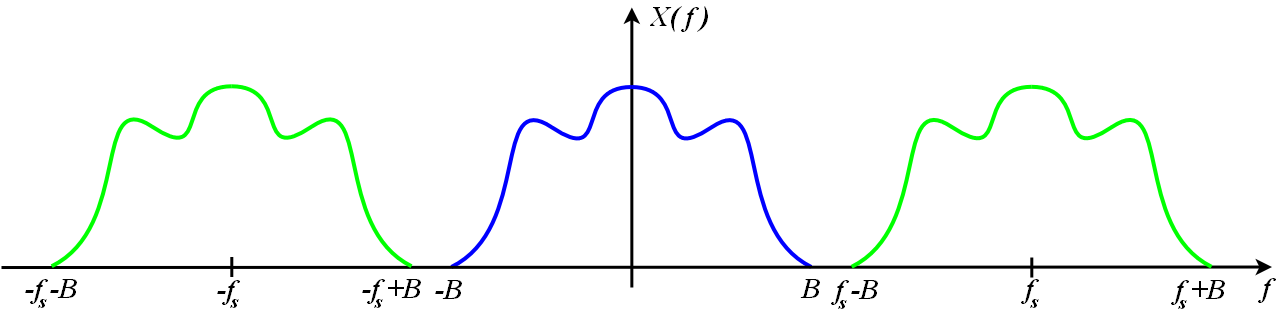
\includegraphics[width=10cm]{sampling.png}
\end{figure}


Aby zrekonstruować sygnał należy odfiltrować nadmiarowe kopie filtrem dolnoprzepustowym i obliczyć odwrotną transformatę Fouriera.
\begin{figure}[h]
    \centering
    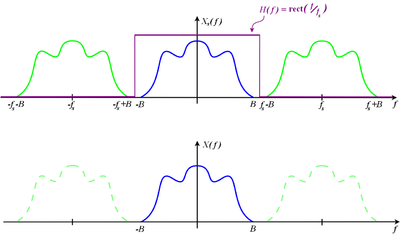
\includegraphics[width=10cm]{sampling2.png}
\end{figure}


Częstotliwość Nyquista - aby poprawnie odtworzyć spróbkowany sygnał częstotliwość próbkowania powinna być większa od dwukrotności najwyższej częstotliwości występującej w sygnale.
\[ f_s > 2f_{max} \]

Gdy częstotliwość próbkowania nie spełnia tego warunku powstanie efekt aliasingu - kopie widma zaczną na siebie nachodzić. Efektem będzie niepoprawnie odtworzony sygnał ponieważ jego widmo zostało zniekształcone swoimi kopiami.
\begin{figure}[h]
    \centering
    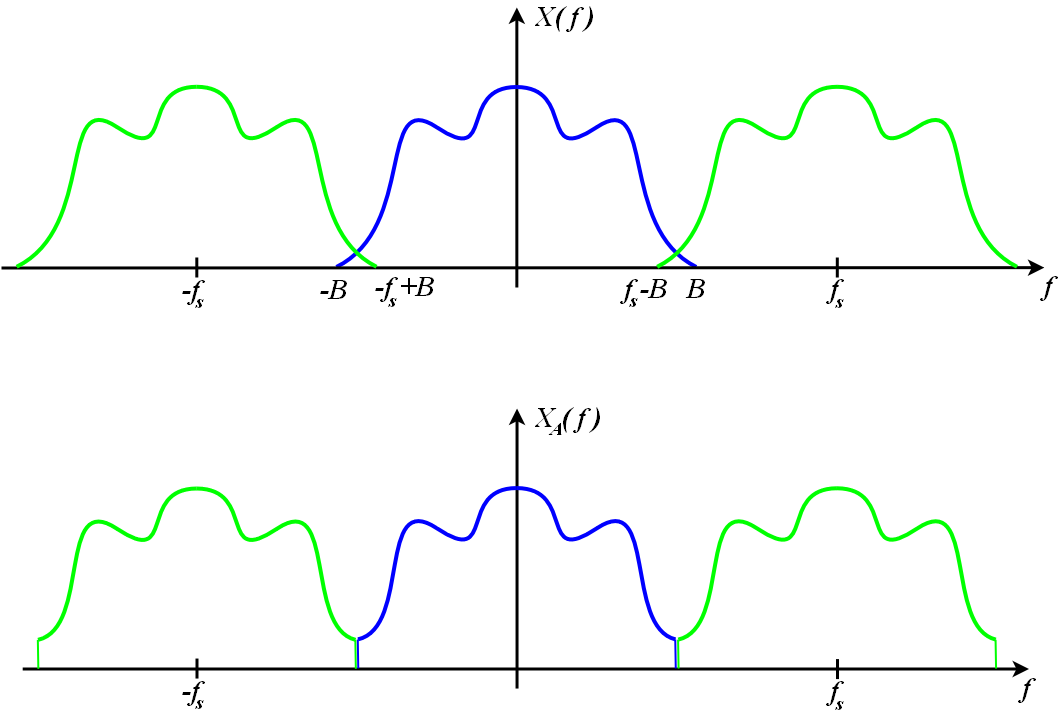
\includegraphics[width=10cm]{aliasing.png}
\end{figure}

\section{Transformacja Z}
\subsection{Wyprowadzenie}
Aby spróbkować funkcję należy ją wymnożyć przez "grzebień" złożony z delt Diraca.
\[ f_d(t) = f(t)\sum_{n=-\infty}^{\infty}\delta (t-nT_s) \]
\[ \mathcal{L} \{f_d(t)\}=\sum_{n=-\infty}^{\infty}f(nT_s) \cdot \mathcal{L} \{\delta (t-nT_s)\} =\sum_{n=-\infty}^{\infty} f(nTs)\cdot e^{-snT_s} \]
Podstawiając $ e^{st_s} = z $ otrzymujemy:
\[ \sum_{n=-\infty}^{\infty} f(nTs)\cdot z^{-n} = \mathcal{Z} \{ f_d(t) \} \]
\subsection{Filtry}
\[ y(n) = \sum_{m=0}^{M}b_m u(n-m) - \sum_{k=1}^{N}a_k y(n-k) \]
\[ y(n) = \sum_{m=0}^{M}b_m U(z)z^{-m} - \sum_{k=1}^{N}a_k Y(z)z^{-k} \]
\[ H(z) = \frac{\sum_{m=0}^{M}b_m z^{-m}}{1 + \sum_{k=1}^{N}a_k z^{-k}} \]

Zera transmitancji odpowiadają za pasmo zaporowe a bieguny za pasmo przepustowe. Bieguny powinny być wewnątrz okręgu jednostkowego (inaczej układ staje się niestabilny) a zera na okręgu jednostkowym (wartości promienia większe od 1 powodują zniekształcenia sygnału). Bieguny i zera można obliczyć z zależności:
\[ \Omega_z = 2\pi \cdot \left( \frac{f_z}{f_s} \right) \]
\[ \Omega_p = 2\pi \cdot \left( \frac{f_p}{f_s} \right) \]
\[ zeros = R_z e^{j\Omega_z} \quad\quad poles = R_p e^{j\Omega_p} \]
gdzie $ f_z $ - częstotliwość pasma zaporowego, $ f_p $ - częstotliwość pasma przepustowego, $ f_s $ - częstotliwość próbkowania

Aby współczynniki transmitancji były rzeczywiste należy przyjąć pary sprzężone biegunów i zer.

\section{Dyskretna transformata Fouriera}
\[ F_k = \frac{1}{N} \sum_{n=0}^{N-1}f(n)\cdot e^{-jk\frac{2\pi}{N}n} \]

Dyskretna transformata Fouriera jest przekształceniem liniowym.

DFT jest obliczana ze skończoną rozdzielczością w dziedzinie częstotliwości - krok zmiany częstotliwości kolejnych harmonicznych wyraża się wzorem:
\[ \Delta f=\frac{f_s}{N} \]
Jeżeli częstotliwość składowej sygnału, na którym obliczmy DFT, nie jest całkowitą wielokrotnością kwantu częstotliwości próbkowania to nastąpi efekt przecieku - pojawią się dodatkowe prążki w dziedzinie częstotliwości.
\begin{figure}[h]
    \centering
    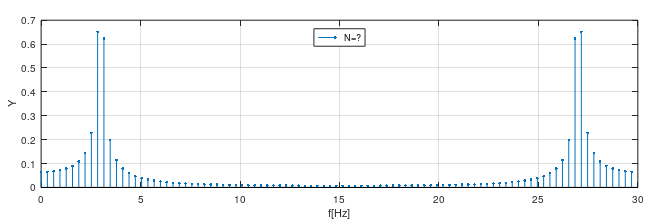
\includegraphics[width=15cm]{przeciek.png}
\end{figure}

Dodatkowo zamiast ujemnych i dodatnich częstotliwości jak w transformacie Fouriera, w DFT występują tylko dodatnie. Samo widmo jest symetryczne a nadmiarowe próbki wynikają z własności splotu kołowego. Należy analizować próbki od 0 do $\frac{f_s}{2}$

Aby zmniejszyć efekt przecieku można wymnożyć próbki sygnału przez funkcję okna np.: impuls trójkątny o szerokości równej szerokości sygnału poddawanego DFT.

\section{Filtry FIR}
Filtry o skończonej odpowiedzi impulsowej - nie zawierają sprzężenia zwrotnego (współczynniki $a_k$ są równe 0.
\[ H(z) = \sum_{m=0}^{M}b_m z^{-m} \]
Zaletą braku sprzężenia zwrotnego jest fakt że taki filtr nie może być niestabilny.
\subsection{Metoda okien}
Algorytm:
\begin{itemize}
	\item Określenie transmitancji na podstawie wymagań
	\item Odwrotne przekształcenie Z na transmitancji
	\item Okienkowanie odpowiedzi impulsowej
	\item $ h_w^M(n) \leftarrow h_w(n-M) $ zapewnienie przyczynowości układu
\end{itemize}
Filtry projektowanie tą metodą charakteryzują się gasnącymi zafalowaniami w paśmie przepustowym i zaporowym oraz liniową charakterystyką fazową w paśmie przepustowym i przejściowym.

Długość odpowiedzi impulsowej jest o 1 większa od rzędu filtru.

Wadą tej metody jest fakt że wynik nie jest optymalny.
\begin{figure}[h]
    \centering
    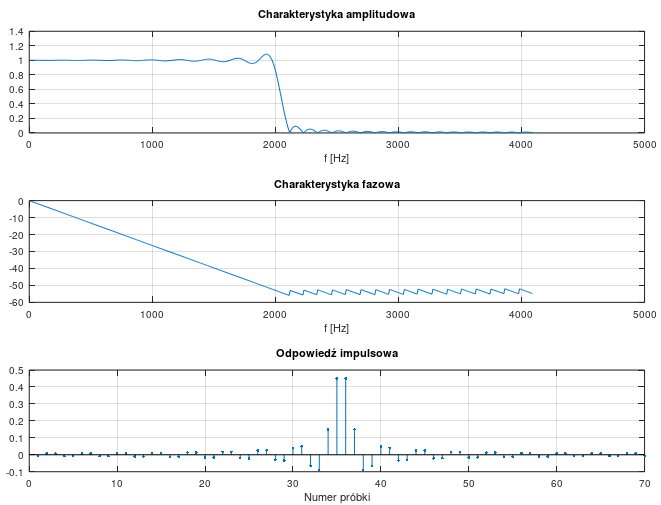
\includegraphics[width=15cm]{fir_ok.png}
\end{figure}

\subsection{Metoda aproksymacji}
Metoda polega na odtwarzaniu zadanego $|H(j\omega|$ za pomocą sumy cosinusów. Dana aproksymacja jest porównywany z zadaną transmitancją i szukany jest minimalny błąd.
\[ \sum_{n} c_n \cos{(n\omega)} - |H(j\omega)| \rightarrow min  \]
Filtry projektowanie tą metodą charakteryzują się niegasnącymi zafalowaniami w paśmie przepustowym i zaporowym oraz liniową charakterystyką fazową w paśmie przepustowym i przejściowym.

Długość odpowiedzi impulsowej jest o 1 większa od rzędu filtru.

Wynik jest optymalny a rząd filtru jest znacznie niższy od rzędu uzyskanego z metody okien.
\begin{figure}[h]
    \centering
    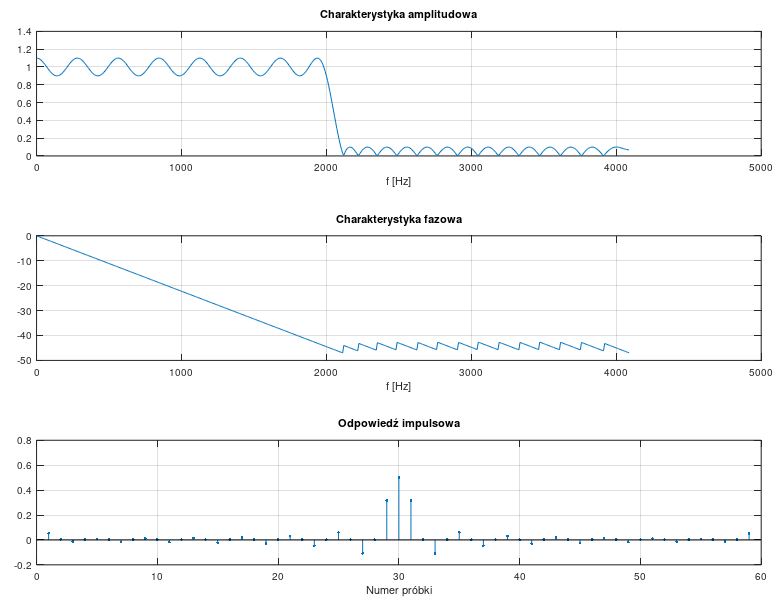
\includegraphics[width=15cm]{fir_ap.png}
\end{figure}

\section{Filtry IIR}
\[ H(z) = \frac{\sum_{m=0}^{M}b_m z^{-m}}{1 + \sum_{k=1}^{N}a_k z^{-k}} \]
Metoda niezmienności odpowiedzi impulsowej - algorytm:
\begin{itemize}
	\item prototyp analogowy
	\item próbkowanie odpowiedzi impulsowej
\end{itemize}

Zaletą filtrów IIR jest brak zafalowań charakterystyki amplitudowej i fazowej oraz znacznie niższy rząd filtru w przeciwieństwie do filtrów FIR.

Wadą natomiast jest nieliniowość charakterystyki fazowej.

\begin{center}
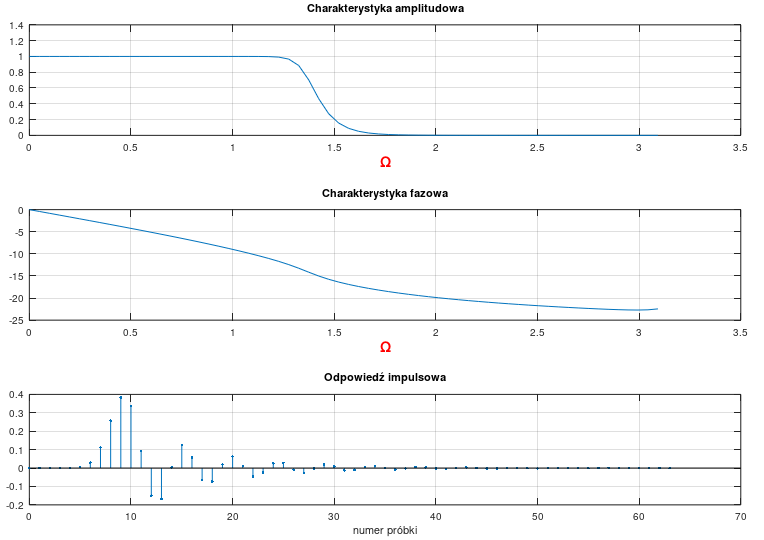
\includegraphics[width=15cm]{iir.png}
\end{center}

\section{Filtry MAV}
Jest to dolnoprzepustowy filtr FIR. Polega na liczeniu średniej z M próbek. Wartość M decyduje o granicy pasma przepustowego. Zwiększanie jej jednak zwiększa także przesunięcie fazowe sygnału.

Filtr ten ma duże zafalowania charakterystyki amplitudowej w paśmie zaporowym przez co słabo tłumi niektóre wyższe częstotliwości. Filtr dobrze nadaje się do usuwania szumu o małej amplitudzie w porównaniu do amplitudy sygnału. 
\begin{center}
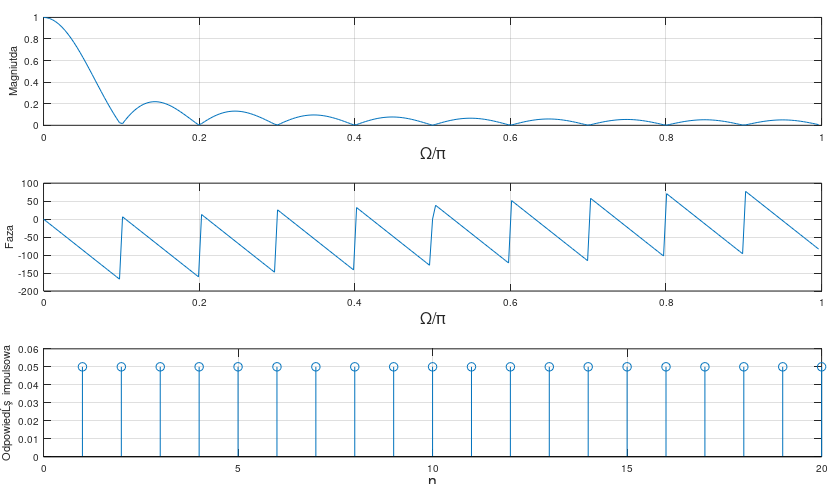
\includegraphics[width=15cm]{mav_ch.png}
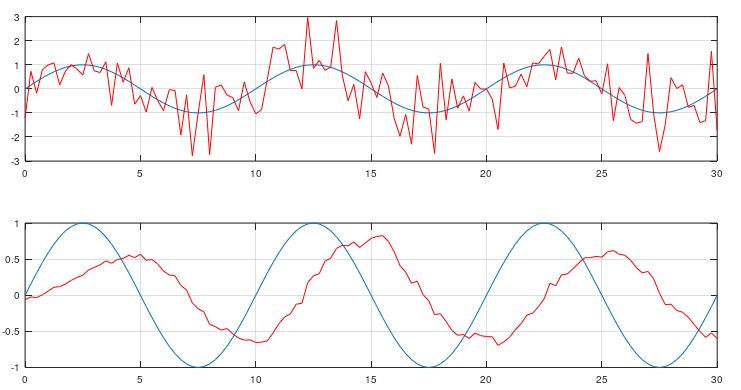
\includegraphics[width=15cm]{mav_g.png}
\end{center}


\section{Filtry CAV}
Filtr ten nadaje się tylko do sygnałów okresowych. Jest to filtr dolnoprzepustowy FIR, który pobiera próbki w tym samym momencie z kilku kolejnych cykli sygnału i oblicza z nich średnią. Sam w sobie nie zapewnia dobrych efektów jednak dobrze "odzyskuje przybliżony kształt sygnału" - zmniejsza się wpływ szumu na sygnał. W połączeniu z filtrem MAV daje dobre efekty.
\begin{center}
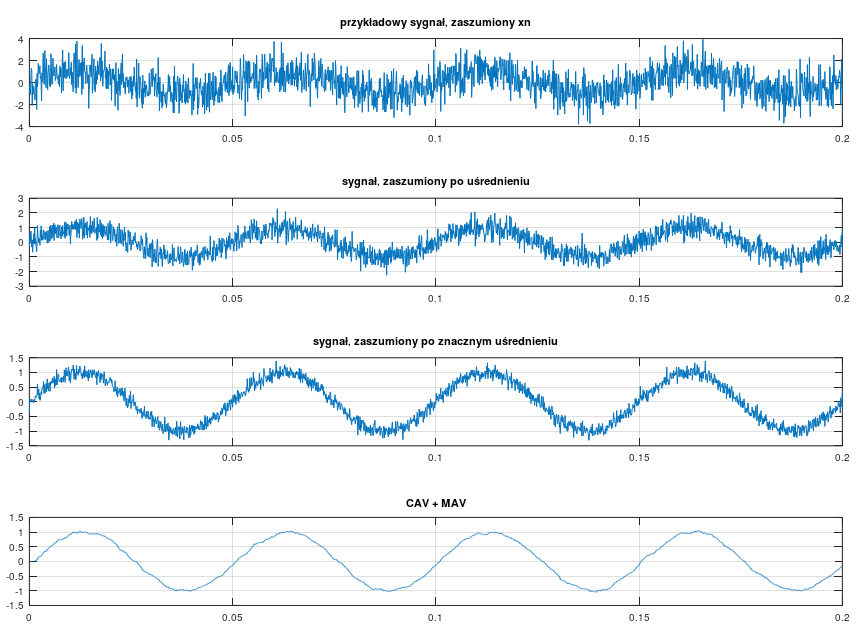
\includegraphics[width=15cm]{cav.png}
\end{center}

\end{document}